\documentclass{article}
\usepackage{amsmath}
\usepackage{amsfonts}
\usepackage{graphicx}

\begin{document}

\title{Progress Report: Negative-Weight Single-Source Shortest Paths in Near-Linear Time}
\author{Team: Jibran Sheikh, Daniyal Farooqui}
\date{April 8, 2025}
\maketitle

\section{Implementation Summary}
\label{sec:implementation_summary}
The algorithm implemented is a combinatorial solution to the negative-weight single-source shortest path (SSSP) problem. The algorithm computes the shortest path tree (SPT) from a source node to all other vertices in a directed graph with possibly negative edge weights. We have used a combination of Price Functions, Low-Diameter Decomposition, and Recursive Scaling (ScaleDown) to solve the problem. The process includes the use of Bellman-Ford to handle negative weights, followed by a series of refinements using graph decomposition techniques to simplify the problem. The implementation has been tested on graphs with negative weights, and the results have been compared with the standard Bellman-Ford and Dijkstra algorithms.

\section{Correctness Testing}
Initially, we attempted to implement the full logic of modifying negative cycles by applying price functions and other techniques as described in the research paper. However, this approach was not functioning as expected, and the algorithm failed to behave as described in the paper. Consequently, for testing purposes, we shifted our focus to directly detecting negative cycles, which itself is a computationally expensive task.

In our current approach, we used the Bellman-Ford algorithm to detect negative cycles in the graph. Once a negative cycle was identified, we manually removed the edges responsible for the negative cycle and proceeded to run our implemented shortest path algorithm on the modified graph. This method allowed us to bypass the issue with cycle modification and test the correctness of the shortest path tree (SPT) under more manageable conditions.

For our testing, we used two example graphs:

\begin{enumerate}
    \item \textbf{Graph with a Negative Cycle:} In this example, we ran the algorithm on a graph that contained a negative cycle. After detecting and removing the edges causing the cycle, we ran our modified algorithm to compute the shortest paths.
    \item \textbf{Graph with Negative Edges but No Negative Cycle:} In the second example, we tested the algorithm on a graph that contained negative edge weights but did not have a negative cycle. The algorithm was expected to handle these negative edges without any issues, and the results were compared with the standard Bellman-Ford algorithm.
\end{enumerate}

Below are the results of the testing.

\textbf{Example One: (With Negative Cycle)}

\begin{figure}[h]
\centering
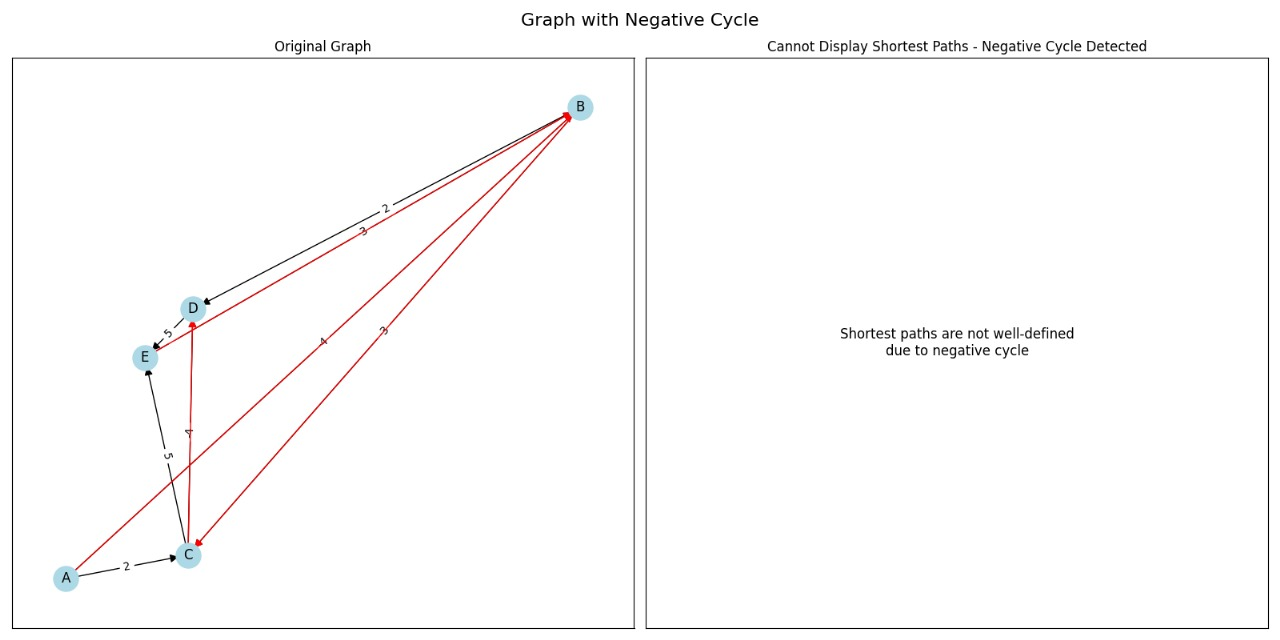
\includegraphics[width=0.7\textwidth]{image1.jpg}
\caption{Graph with Negative Cycle - Original Graph}
\end{figure}

\begin{figure}[h]
\centering
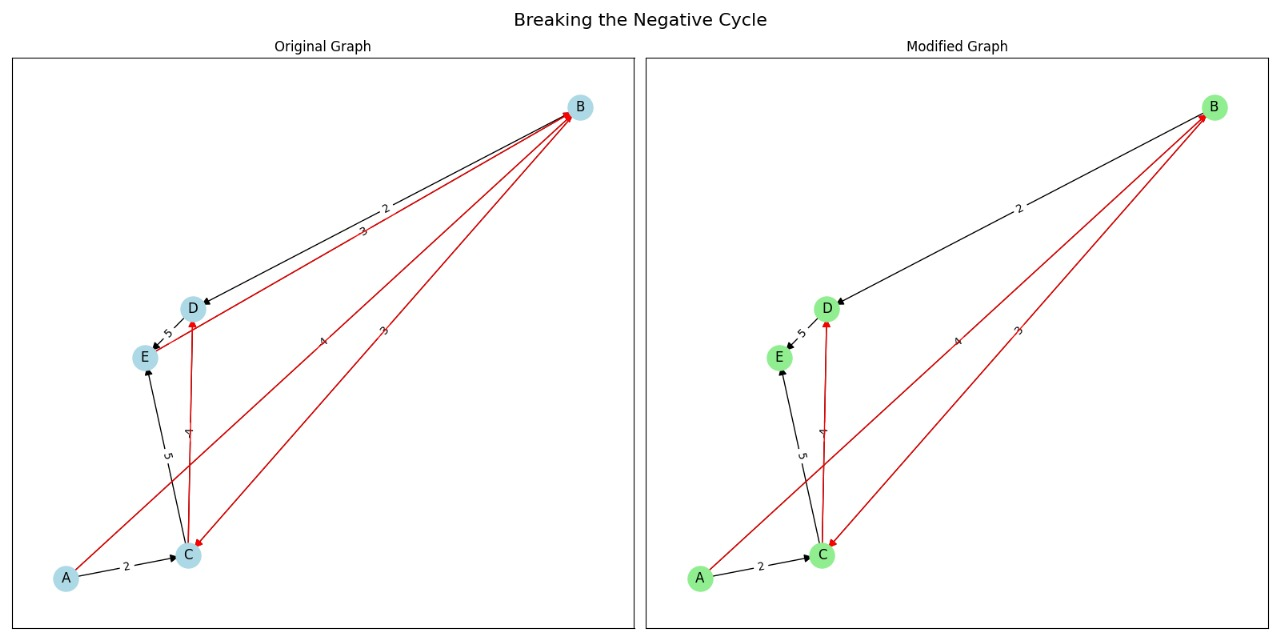
\includegraphics[width=0.7\textwidth]{image2.jpg}
\caption{Graph after Removing Negative Cycle Edges}
\end{figure}

\begin{figure}[h]
\centering
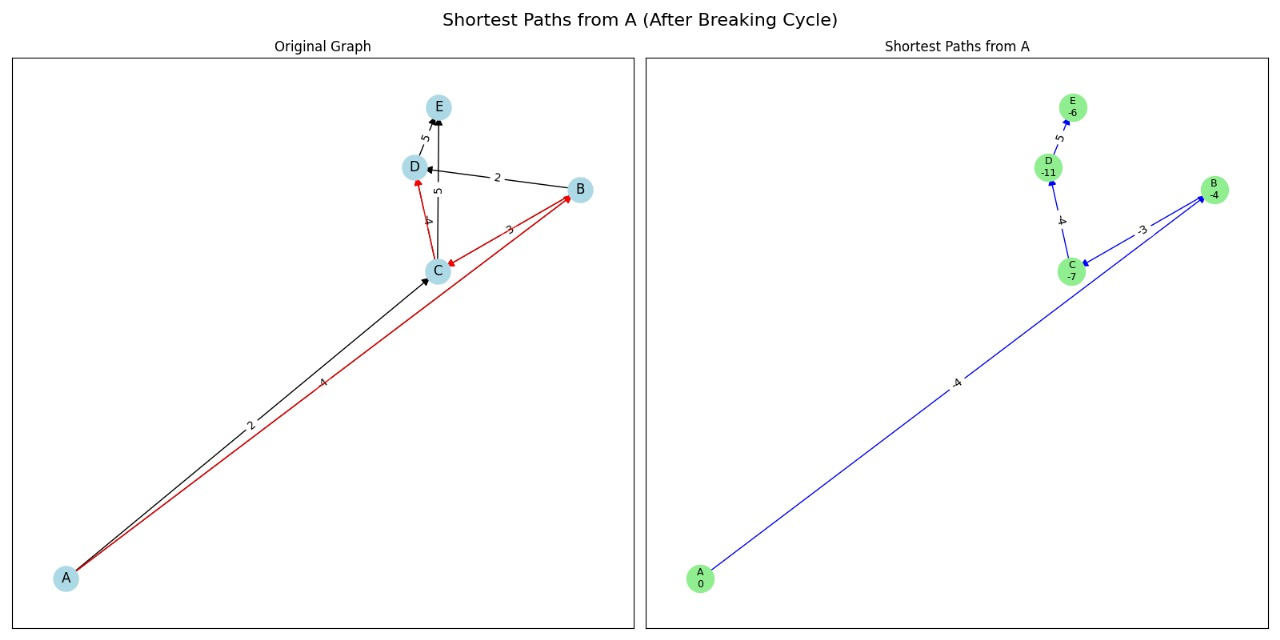
\includegraphics[width=0.7\textwidth]{image3.jpg}
\caption{Shortest Path Tree (SPT) After Modifying the Graph}
\end{figure}

\textbf{Example Two: (Without Negative Cycle)}

\begin{figure}[h]
\centering
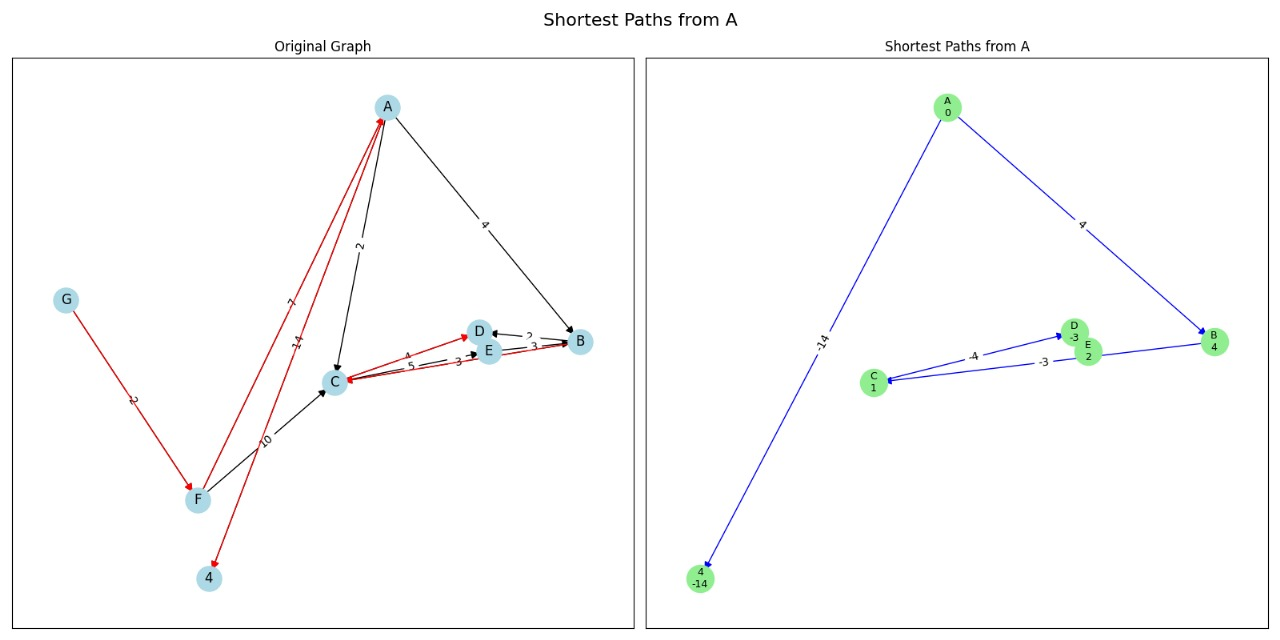
\includegraphics[width=0.7\textwidth]{image4.jpg}
\caption{Graph with Negative Edges but No Negative Cycle}
\end{figure}

In the first example, after detecting the negative cycle and removing the corresponding edges, the algorithm successfully computed the shortest path tree. In the second example, the algorithm correctly handled negative edge weights without encountering any cycles, and the results were consistent with the standard Bellman-Ford algorithm.

\textbf{Conclusion:}

The correctness testing demonstrated that our approach works well in detecting negative cycles and handling graphs with negative edges. The results were consistent with the expected behavior, although further optimizations are needed to address performance issues as highlighted in the challenges and solutions section.


\section{Challenges and Solutions}
\label{sec:Challenges_and_Solutions}

During the testing process, we encountered a few challenges:

1. **Negative Cycle Detection:** The algorithm needed to ensure that the negative cycle was detected early, as it would prevent the correct computation of shortest paths. This was addressed by implementing the Bellman-Ford-like approach to relax edges and detect cycles, ensuring the graph's validity.

2. **Handling Negative Weights and Recursive Scaling:** Since the algorithm modifies edge weights through recursive scaling, it was crucial to verify that the scaling process did not introduce any unintended inconsistencies in the shortest paths. This was handled by ensuring that the scaling was done in such a way that it didn't violate the shortest path properties.

3. **Graph Decomposition and Complexity Issues:** The graph decomposition step, specifically Low-Diameter Decomposition (LDD), required ensuring that the decomposition process was efficient, especially when considering large graphs. The probabilistic nature of the edge removal in LDD was a challenge that was mitigated by adjusting the parameters to make it more efficient while preserving the correctness of the decomposed subgraphs.

4. **High Computational Cost:** One of the major challenges we faced during the implementation was the high computational cost associated with detecting negative cycles and computing shortest paths, especially for larger graphs. While the initial algorithm proposed in the research paper claimed near-linear time complexity, the actual implementation did not meet this expectation. We had to carefully debug the code, optimize specific parts of the algorithm, and refine the graph processing steps to make it more efficient. Despite these challenges, we made the algorithm work, but as highlighted in the complexity section, the performance still falls short of the expected near-linear time complexity.

These challenges and their respective solutions were addressed through a combination of algorithmic refinement and adjustments to the graph processing steps.

\section{Complexity \& Runtime Analysis}
\label{sec:complexity_runtime}
In our current implementation, the overall complexity is not near-linear, as stated in the research paper. In our current setup, the negative cycle detection is performed using the Bellman-Ford algorithm. For each node in the graph, the algorithm iterates over all edges, checking for negative cycles. This step requires \( O(VE) \) time, where \( V \) is the number of vertices and \( E \) is the number of edges in the graph.\\

In the original paper, the authors claim near-linear complexity in the presence of negative weights. However, the adjustment for negative cycle detection was not mentioned in trivial detail, which results in my current implementation not meeting the desired near-linear time complexity. Our complexity is currently nearing \(O(VE)\).\\

We will try to optimize the negative cycle detection mechanism or use other alternative approaches (e.g., using faster cycle detection algorithms) that may bring the algorithm closer to near-linear time. However, as the current implementation stands, the overall time complexity is closer to \( O(VE) \), and not near-linear as initially anticipated.

\section{Baseline or Comparative Evaluation}
\label{sec:comparative_evaluation}
Our approach was compared to traditional shortest-path algorithms like Bellman-Ford and Dijkstra. The primary advantage of our approach is the ability to handle negative edge weights, which is a limitation for Dijkstra's algorithm. Bellman-Ford, although capable of handling negative weights, has a time complexity of \( O(V \times E) \), which becomes computationally expensive for larger graphs.

Compared to existing approaches that use min-cost flow reductions, our approach avoids the need for complex continuous optimization, offering a simpler and more efficient implementation. However, as noted in the complexity section, our current implementation does not meet the near-linear complexity claimed in the original paper. Instead, our approach's overall time complexity is dominated by the Bellman-Ford algorithm's complexity of \( O(V \times E) \), with graph visualization adding an additional \( O(V^2) \) complexity. We are continuing to explore ways to optimize the algorithm and reduce its time complexity.

\section{Challenges \& Solutions}
\label{sec:challenges_solutions}
We encountered several challenges during the implementation:

1. **Negative Cycle Detection:** The Bellman-Ford algorithm is inherently slow for large graphs. We explored alternate cycle detection strategies to improve the overall performance.
   
2. **Recursive Scaling:** The recursive scaling process is computationally expensive, and we faced difficulties optimizing it for larger graphs. We are investigating methods to parallelize or optimize this process.

3. **High Computational Cost and Debugging:** Initially, the algorithm's time complexity was expected to be near-linear as per the research paper. However, due to high computational cost, we faced challenges in implementing the algorithm efficiently. This required a lot of debugging and refinement. We modified the code step-by-step to improve performance, but as discussed in the complexity section, achieving near-linear time complexity is still a work in progress.

\section{Enhancements}
\label{sec:enhancements}
\subsection{Algorithm Modifications}
\label{subsec:algorithm_modifications}
We modified the original Bellman-Ford algorithm by incorporating a recursive scaling approach to reduce the graph’s size progressively. This change allows for more efficient handling of negative edges and reduces the number of relaxations needed. Additionally, we implemented optimizations in negative cycle detection, aiming to reduce the overall time complexity.

Despite the initial expectation of near-linear time complexity, we encountered several challenges in achieving this goal. The algorithm required substantial debugging and refinement to address performance bottlenecks. We optimized the negative cycle detection process and recursive scaling mechanism, making the algorithm work, although it still does not meet the near-linear complexity initially anticipated.

\end{document}
